\section{Cavers returning}

\begin{marginfigure}
\begin{tikzpicture}
\node [name-dest] (box){%
    \begin{minipage}{0.80\textwidth}
     \begin{itemize}
    \item Tanguy Racine
    \item Aileen Brown
    \end{itemize}
    \end{minipage}

};
\node[fancytitle, right=10pt] at (box.north west) {A Pun Too Far};
\end{tikzpicture}
\end{marginfigure}

\textit{The following article was in part published in the student newspaper of Imperial College London \smallcaps{Felix} after the return of the 2014 expedition. In each of its weekly issues, a couple of pages are dedicated to the goings-on of clubs and societies within the College.}

\mydelimiter

`Hey ho!' 

Silence...  We knew what it meant. Cavers returning. 

The kettle let out a loud hisssss and started shaking and gurgling.. The sound of a tackle bag falling heavily on the floor. 
We all looked up. `Hey ho!'

And interrupted conversations resumed, `Yes this word fits'

`What about fifteen down?'

`Does it go?'

`Tea is up!'

`Where's the cow?'...

I was sat in the bivi, a large surface depression with an overhanging rock bridge on the \passage{Migovec} Plateau in the \passage{Triglav National Park}, western Slovenia. From the `\passage{Sunset Spot}' I could see all the way to Italy and on a clear sunset we could even spot the Dolomites rising in the distance, crowned with russet light. West of \passage{Migovec} is the \passage{Krn} massif, a former war front during WWI, which I observed many a time wreathed in storm clouds while stars twinkled upon \passage{Migovec}.


\begin{marginfigure}
\checkoddpage \ifoddpage \forcerectofloat \else \forceversofloat \fi
\centering
\frame{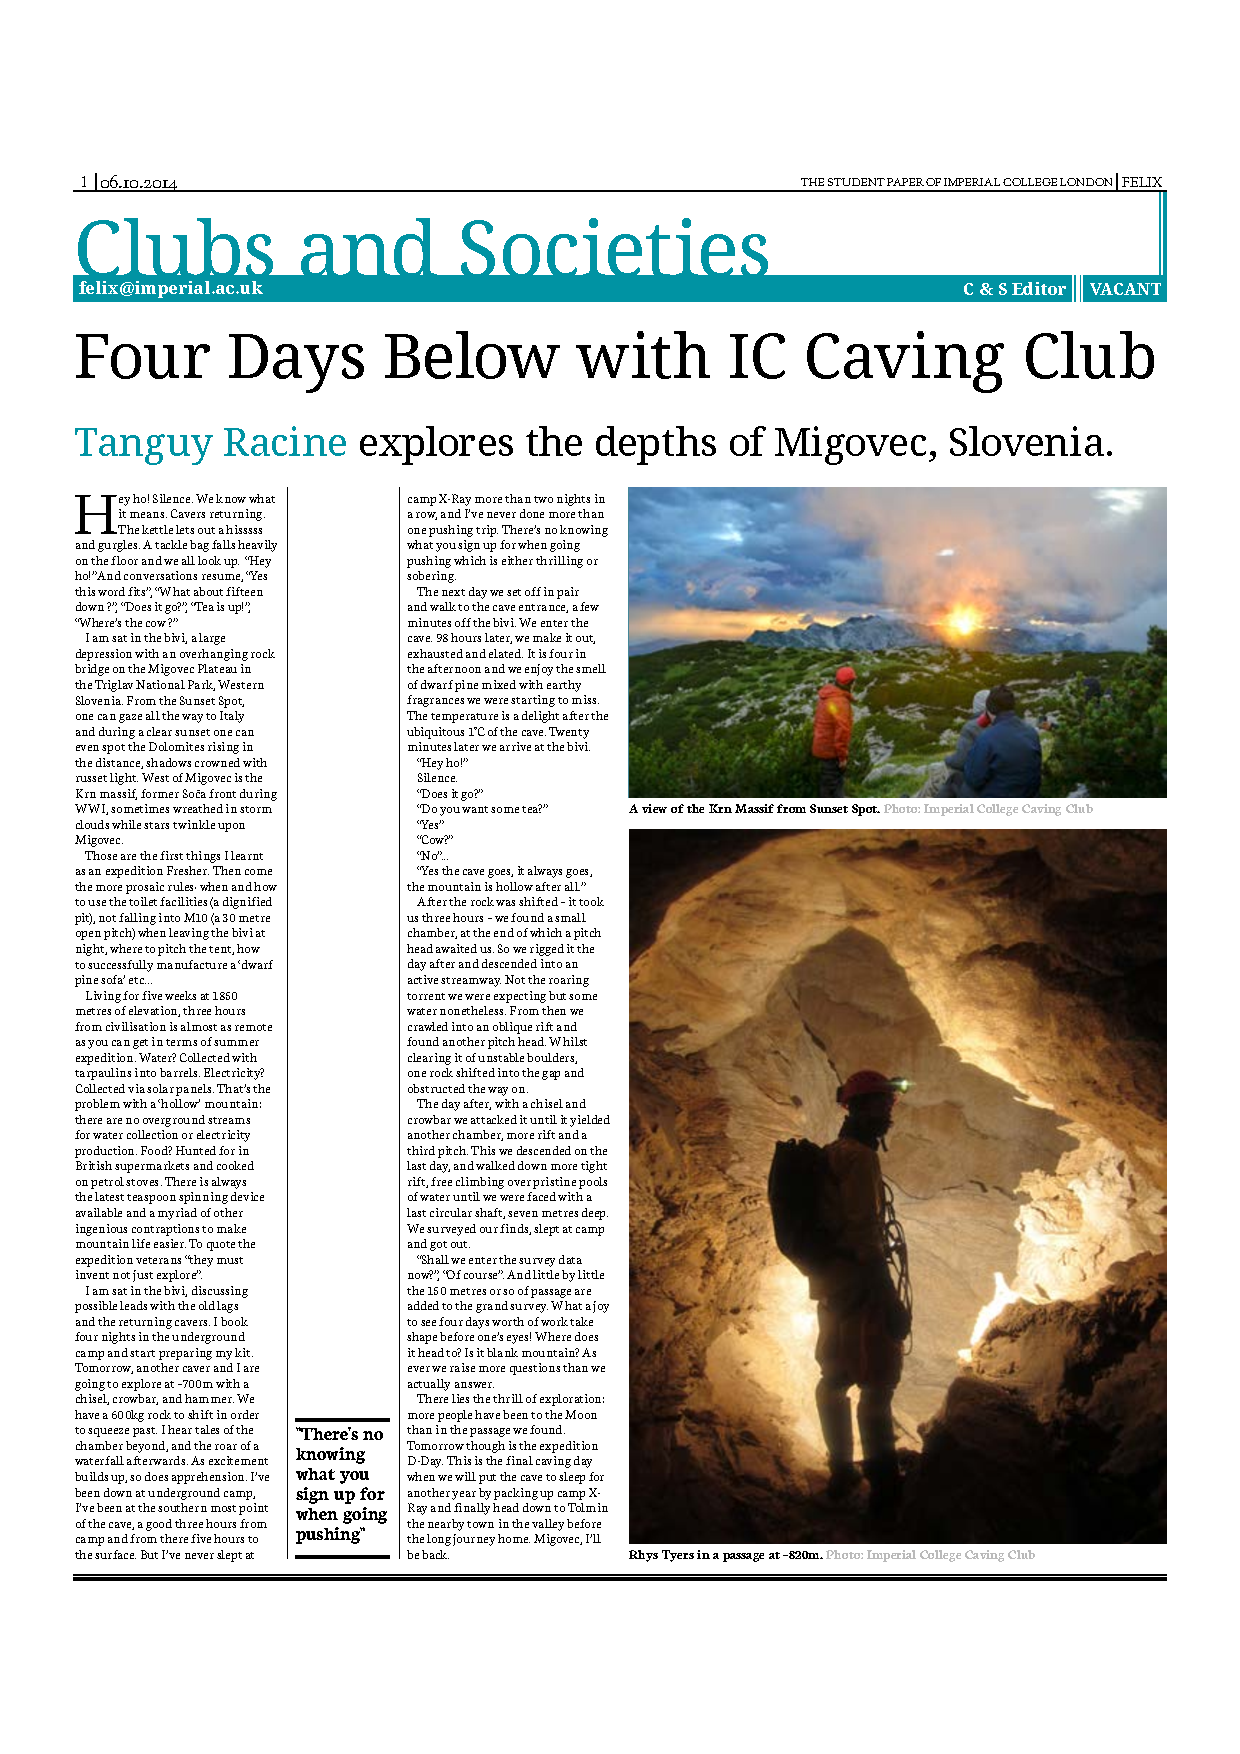
\includegraphics[width=0.99\textwidth]{images/2014/tanguy-2014/felix_1583_oct_12_2014.pdf}}
\caption{Felix issue 1583, 12th October 2014, p30 --- Tanguy Racine}
\label{felix article}
\end{marginfigure}

There were a few things I learnt as an expedition Fresher. First the more prosaic rules: when and how to use the toilet facilities (a dignified pit), not falling into \passage{M10} (a 30 metre shaft open to the surface) when leaving the bivi at night, where to pitch the tent, how to successfully manufacture a `dwarf pine sofa' etc... 

Living for five weeks at 1850 metres of elevation, three hours from civilisation was almost as remote as you could get in terms of summer expedition. There is a catch with karstic terrain though: there are no overground streams for water collection or electricity production. So the water is collected with large tarpaulins into barrels, or melted from shakehole snow plugs - a tiresome business. Electricity? solar power channelled to recharge drill batteries.  Food? Hunted for in British supermarkets and cooked on petrol stoves. Confort? there is always the latest teaspoon spinning device available alongside a myriad of other ingenious contraptions to make mountain life easier. To quote the expedition veterans 

\begin{quote}` they must invent not just explore'\end{quote}

We had passed the midpoint of the expedition, and I was sat in the bivi, discussing possible leads with the old lags and the returning cavers. I booked four nights in the underground camp and started preparing my kit. On the morrow, Aileen, an Irish caver and I were going to explore at -700m, equipped with chisel, crowbar and hammer. We had a half-ton rock to shift, then squeeze past and find the continuation. Hanging around in the bivi, I kept hearing tales of the chamber and its roaring waterfall beyond and as excitement started building up, so did the apprehension. I'd been down at underground camp before. I'd been at the then southernmost point of the cave, a good three hours from camp and from there five hours to the surface. But I'd never slept at camp \passage{X-Ray} more than two nights in a row, and I'd never done more than one 'pushing' trip. 
There was no knowing what you signed up for when going to the pushing front; to an 18 year old with its head full of dreams of glory is thrilling. So, I had to look back at what I'd done during the early weeks of expedition.

\mydelimiter

\begin{figure*}[t!]
\checkoddpage \ifoddpage \forcerectofloat \else \forceversofloat \fi
\centering
\frame{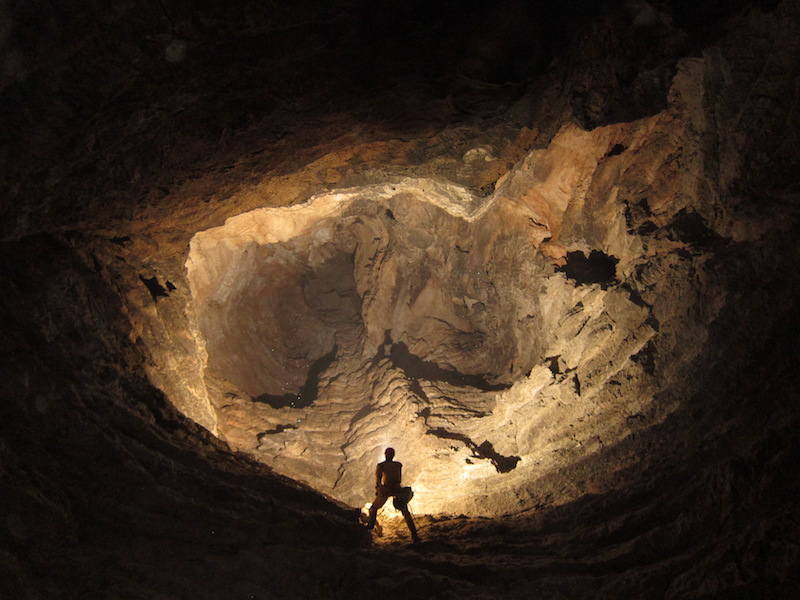
\includegraphics[width=0.99\textwidth]{images/2014/tanguy-2014/bottom_of_pico.jpg}}
\caption{Bottom of Pico pot --- Jarvist Frost}
\label{Pico}
\end{figure*}



\section{A Fresher's first camping trip}

\begin{marginfigure}
\begin{tikzpicture}
\node [name-dest] (box){%
    \begin{minipage}{0.80\textwidth}
     \begin{itemize}
    \item Tanguy Racine
    \item Rhys Tyers
    \end{itemize}
    \end{minipage}

};
\node[fancytitle, right=10pt] at (box.north west) {Sic Semper Tyrannis};
\end{tikzpicture}
\end{marginfigure}

My first camping trip took me to the southernmost end of the system, a good eight hours from the surface, at a depth of -800m. It had been left two years ago as a potential lead at the end of the \passage{Atlantis} passage, where two equally inviting passages forked. 

\label{sec:helmsdeep}

The right-hand one had been pushed and surveyed to a perched sump ( \passage{Lethe} ) the year before, but the flat out crawl to its left hadn't been properly examined, although it was repeatedly remarked that a `way on was visible'. 

The end of \passage{Atlantis} lies approximately 500m due south of the cubic kilometre of dense tangled network, into completely blank mountain. Although it is mostly stooping or walking passage,it must be stressed how far this lead is from camp, let alone the surface.


\begin{marginfigure}
\checkoddpage \ifoddpage \forcerectofloat \else \forceversofloat \fi
\centering
 \frame{\includegraphics[width=\linewidth]{"images/2014/tanguy-2014/laurel-jarv".jpg}} 
 \caption{Rhys Tyers, ascending the upper section of \protect\passage{Laurel} pitch ---Jarvist Frost}
 \label{Laurel-up}
\end{marginfigure}

On the surface, I checked twice to make sure I had every bit of my SRT kit and then looked around. Clouds were rising from Gardeners' World valley, and drifting towards \passage{Vrh Nad Skrbino} peak with a menacing look. I quickly put my bag underneath the rock lip, by the entrance to the cave. Rhys and I had been on the first rigging trip of the year down to the top of \passage{Tesselator}. I'd rather enjoyed walking on a thin rock promontory to descend the wet route down \passage{Laurel} and getting rebelay practice down \passage{Pico}.

This time when we entered the cave, I noticed the mists rising from our lips. Down, down, down we went. Keeping a good pace, we reached the bottom of \passage{Swing} and the deepest I had been in the cave so far. Rhys, wriggled through the tight \passage{Tesselator} pitch head like an eel, rigged his descender and quickly said `that was the technique to get past, now do the same, and we'll meet at the bottom of the shaft series'. He disappeared, singing.

I obliged, and descended. Pitch after pitch, \passage{Space Odyssey}, \passage{Concorde} etc? I had seen those names on the survey, in fact I'd peered over the laminated copy kept in the bivi many a time, wondering, trying to remember the photographs on the first slideshow I had seen several months ago when I joined ICCC.




Depth clocked up quickly now, and in no time we arrived at camp \passage{X-Ray}, where Rhys went straight for a little square of white paper and showed it to me. It read:

\begin{quote}
`Welcome Team 2014, push hard and good luck!'
\end{quote}

He'd written it the year before as \passage{X-Ray} was put to sleep for the Winter Months. It was our job to set it back up and running for the several hundred man-hours spent there during the expedition. 

First, flatten the surface for sleeping. We clambered further down \passage{Friendship Gallery} to fill tacklesacks with sand and pour the stuff over the sleeping area, which after a few comings and goings began to  resemble a flat surface. We left one rock poking up at one corner, ot provide Dave Kp with a pillow. 

That done, Rhys brewed a cloudy, gritty tea. I don't take milk in tea at the best of times, but having half dissolved milk powder (Nido) with a silty froth (macchiato, says Rhys) as the only available warm drink forced me to re-evaluate my stance. Warmth was welcome though, and soon music was on, as well as a copious dinner. William and Sam, announced themselves with a muffled 'Rope free' in the nearby \passage{Zimmer}, and the usual rattle of SRT and arrived shortly after with the rest of the camp's logistics, sleeping bags and 'comf'. The tent which had been hanging upside down was upturned and almost as quickly filled with a human presence. 

\begin{figure*}[t]
\checkoddpage \ifoddpage \forcerectofloat \else \forceversofloat \fi
\centering
\frame{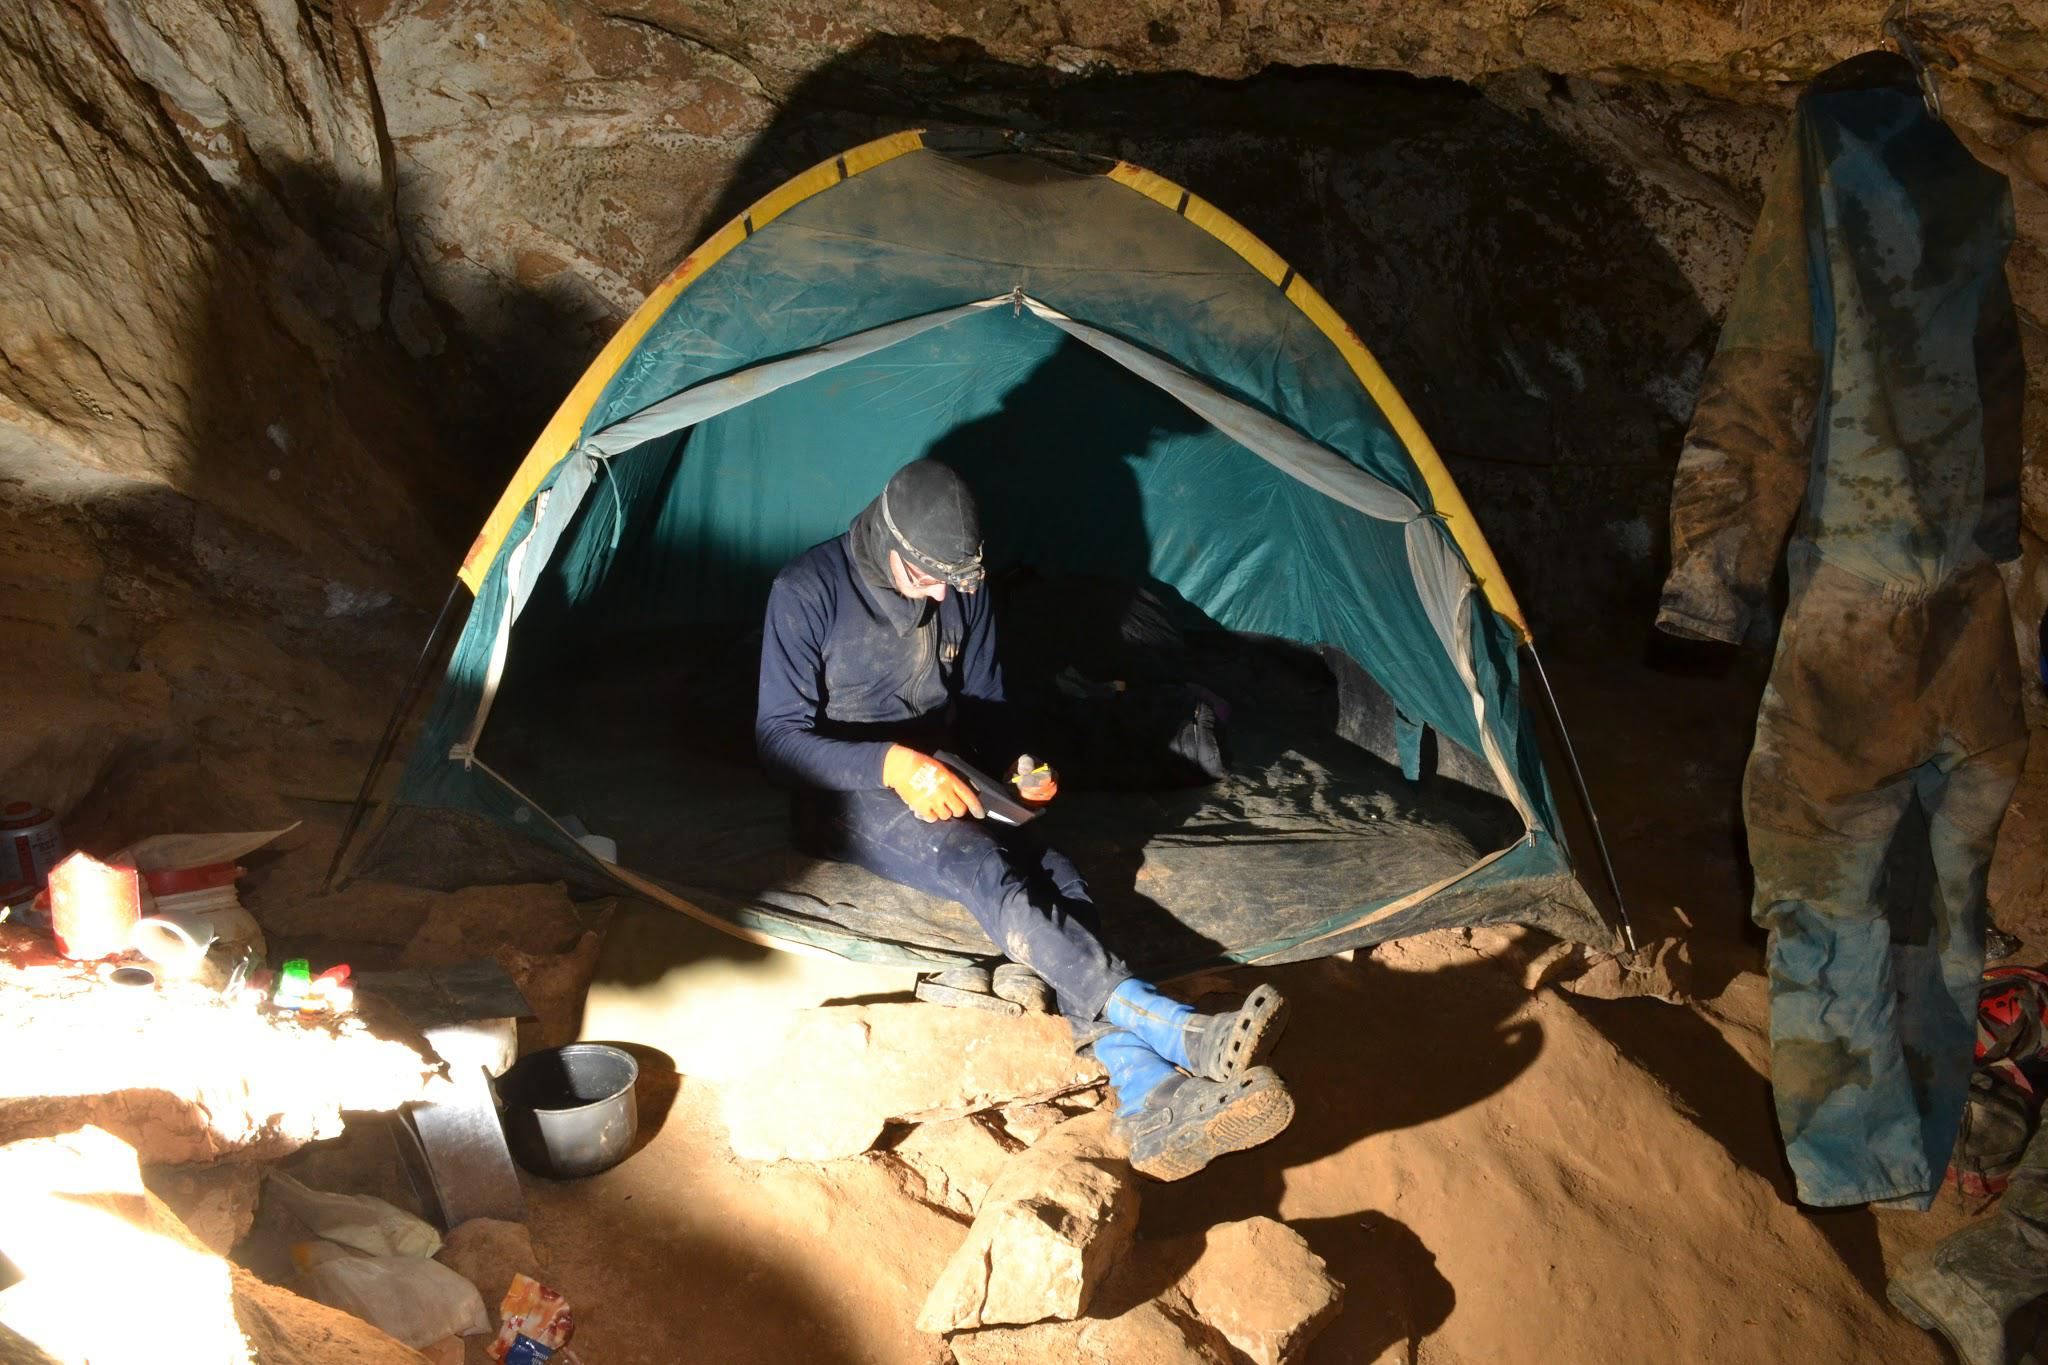
\includegraphics[width=\textwidth]{images/2014/tanguy-2014/camp_x-ray.jpg}}
\caption{Writing in the log book at Camp X-Ray --- Rhys Tyers}
\label{Camp X-Ray}
\end{figure*}



We drifted to sleep... A hungry stomach, and somewhat sore back saw to my waking up in the absolute darkness and did a good job at occupying my thought process during those crucial minutes. 
The underground way of life came quite naturally as I put a pan on the fire and rummaged behind a big rock in search of adequate breakfast food. A meal was soon ready, and we wolfed it down. Then I felt the sleeves of my fleece undersuit: they were mildly damp. The same was true of the gloves and the wetsocks. Rhys, ruminating the same thoughts, exclaimed `Now for the worst part of your daily routine: putting wetsock one and wetsock two'. 

\recipecorner{Biopork savoury rice}{A particularly scrumptious UG special
\begin{citemize}
\item Cut chunks of pork
\item Fry with pork pâté and onions
\item  Bring water to boil with savoury rice
\item Add savoury sachets to taste
\item Cut up cheese medaillons 
\item Mix rice and pork chunks
\item Add medaillons at last minute and savour hot!
\end{citemize}
}

 Five minutes later though, with welly boots on and blood circulation warming them a bit we were as ready as we were likely to get, so we set off for the southern reaches of the System. 
 


We climbed up, into the deep, dark cleft at the bottom of \passage{Zimmer} and soon descended the muddy and loose \passage{Cheetah} pitch. Some three or four challenging (for a fresher) rebelays later, I was swinging at the bottom hang to land on a balcony. The pitch had intercepted a wide horizontal passage. Rhys pointed at the dark space beyond the pitch, at the other window saying: `this is the way to the connection'. 

\begin{figure*}[b!]
	\begin{tikzpicture}
	\node [name-dest] (box){%
		\begin{minipage}{\textwidth}
		\begin{multicols}{2}
		We're back! \passage{Atlantis} goes! Following on from a turn off to \passage{Brezno Slapov} a flat out squeeze leads immediately to a sort of shattered phreatic passage. We got ~170m before hitting a waterfall and a large chamber. There's a big draught round there and quite a few leads off that we didn't look at. I had an incredibly enjoyable trip today. Tanguy continues to be good company (and a fast surveyor) and accompanying our exploits with LOTR soundtrack gave it a very epic feel.
		\name{Rhys Tyers}
		\end{multicols}
		\end{minipage}};
	\node[fancytitle, right=10pt] at (box.north west) {Logbook extracts: Sic Semper Tyrannis};
	\end{tikzpicture}
\end{figure*}

Rhys was a very helpful guide as he described every junction we faced. `Put your feet here', 'look around so you remember which way to go on the way out' 'If you go that way you walk for fifteen minutes until you hit a dead end' etc... We found another very muddy pitch on the way, \passage{Stuck in Paradise} it was called and apparently it was far better now than when first discovered.At the time, I made a mental note to find a bypass as one of the expedition's aims \sidenote{this did not prove successful, although the author was teased for the discovery of a potentially worse bypass, which remains unpushed at the time of writing}. 


It was again, a very slippery and muddy pitch, and, as I was to later find out to Sam's expense, horrifically loose. Some of the rigging looked very tight and I spent a good ten minutes trying to recover from a braking carabiner jammed in my descender krab. When footholds are scarce, hanging rebelays are lonesome places at the best of times. But seven hundred metres down, with nothing but mud to hang on to, they are objectively challenging. Cursing and muttering I finally freed myself through brute arm strength.

\begin{figure*}[t!]
\checkoddpage \ifoddpage \forcerectofloat \else \forceversofloat \fi
\centering
    \begin{subfigure}[t]{0.393\textwidth}
        \centering
        \frame{\includegraphics[width=\linewidth]{"images/2014/tanguy-2014/rhystyers_amazinggrace-2__1_".jpg}} 
        \caption{} \label{HelmsDeep}
    \end{subfigure}
        \hfill
\begin{subfigure}[t]{0.59\textwidth}
\centering
\frame{\includegraphics[width=\linewidth]{"images/2014/tanguy-2014/rhystyers_amazinggrace__1_".jpg}}
 \caption{}\label{water chamber below helm's deep}
\end{subfigure}
    \vspace{0cm}
    \begin{subfigure}[t]{\textwidth}
    \centering
        \frame{\includegraphics[width=\linewidth]{"images/2014/tanguy-2014/rhystyers_atlantis__1_".jpg}} 
        \caption{} \label{Atlantis}
    \end{subfigure}
    \caption{
    \emph{(a)} The roped climb up into \protect\passage{Amazing Grace}.  
     \emph{(b)} \protect\passage{Puff the Magic Dragon} a classic bedding controlled phreatic passage
     \emph{(c)} Phreatic passage decorated with stalactites in \protect\passage{Atlantis} --- Rhys Tyers }
\end{figure*}

Down the pitch we found \passage{Hawaii} junction and a cache for Darren drum, mess tin and a few lengths of red `9 mil rope'. Time for a little break and history lesson. 

\fref[margin]{sec:creature}
There, Tetley and Sam had been assailed by a trogloxene creature, a mammal, as large as a bear, as cunning as a fox, or as adorable as a cat depending on the stories. Fighting for their lives, they had later brought back some food to offer up to the cave gods on the \passage{Hawaii} altar. And hours later, the gods had taken their due (or else hid it under a rock). 


I had a look at the Daren drum left at the junction for collecting the drips. Overall, this region of the cave was quite dry. It was at least 500m from any running water in all directions, and fenced by an incredibly muddy pitch to the west, a knee-killer crawl to the east. The southern passage, ie: the \passage{Atlantis} extension was the longest, with various crawls and squeezes to get past. I started to grasp why there were so much logistical hurdles involved exploring these remote environments.

I was less impressed when I unscrewed the lid of the Daren drum though: a brown layer of silt had settled out of suspension at the bottom, over 11 months, but as I moved the keg, it all mixed up again. Luckily I had a water bottle with me, and it was half full.

Rhys looked around, and showed the uninviting offshoot to \passage{Hash}. `The entereable section ends in a dogleg even Clare was scared of...' That said it all. We carried on, until we found the boulder choke at the end of \passage{Lost Miles}. Off came the SRT kit, and we squeezed through. 
Then began \passage{Atlantis} \emph{stricto sensu}. The cluster of stalactites and muddy stalagmites was there, as Rhys had promised: they were one of the rare formations in \passage{Migovec}. 

We were on the lookout for a passage leading off to `\passage{We're Not Alone}' to our left, which Dave had talked about. It was a very obvious beckoning dark hole when coming back from the pushing front, less so on the way there, but we only stood peering at the blackness beyond, trying to fathom the distance the passage went, to little avail. We could have just walked the few metres, but instead, we pressed on. Down and further south still. The ceiling lowered gently to a little sandy and pebbly crawl, which led to a bigger chamber and then, the boulder choke.

\begin{marginsurvey}
	\includegraphics[width= \linewidth]{"images/little_insets/sicsemper_inset".pdf}
	\caption[Sic Semper Tyrannis]{Plan view of the \protect\passage{Sic Semper Tyrannis} passages beyond \protect\passage{Atlantis} --- Slovenian National Grid EPSG 3794}
\end{marginsurvey}


With a little hesitation about what where the lead actually was, we negotiated the flat out crawl. After a sharp bend it opened up and turned to walking phreatic passage with a strong draught. One large ledge protruded from each side, providing a path 1.5 metre from the ground with mud ripples on the upper surfaces as well as multiple other mud formations. It continued for 20 metres to an alcove on the left, and a pit to the right. Climbing into the alcove we followed a tunnel shaped, sandy passage until we hit a junction, 15 metres on. 

Now grinning broadly, we pushed the lead northward and upwind until once again, a pit appeared on the right before a turn to the left. It seemed never to end and every pit, or junction opened more possibilities. I was thrilled. It was, by any standards a great find for a first pushing trip, because we'd left more leads than we started with; good leads they were too. I started thinking about finding our way back, perhaps I was far too keen at that point, and started building a cairn with elongate cobbles indicating the path we'd come from. 

\begin{survey}[t!]
\checkoddpage \ifoddpage \forcerectofloat \else \forceversofloat \fi
\centering
\frame{\includegraphics[width=\textwidth]{"images/2014/tanguy-2014/sic_semper_tyrannis".png}}
\caption[Sic Semper Tyrannis (grade 1)]{Grade 1 sketch of Sic Semper Tyrannis recorded in underground logbook --- Rhys Tyers}
\label{G1 sketch}
\end{survey}

Rhys on the other hand left little notes with helpful messages and tips on such as 'pitch undescended as of 21st Sept and so on. Having turned left from the pitch head (we had no rope), there was an awkward pit traverse. I free climbed down to check for any leads, and I believe there is one \sidenote. Instead, we chose the more obvious passage after the pit. Whenever it seemed to close down there was an obscure way on. We passed two sandy circular chambers separated by constrictions. This led to a larger chamber with a boulder floor sloping toward the north, with bit of a free climb to go down. 

At the western end the draught disappeared through another constriction from which the trickle of water could be heard. The passage ended 10 metres later at the foot of a 5 metre high waterfall. The water pooled at the bottom before flowing eastward through the boulders. A way on could be seen from there, underneath the pile of boulders, but it wasn't checked this year. Content with the amount of passage found so far we decided to start the surveying of the chamber. Since we were both presidents, (I was president elect at the time) we settled upon the name \passage{Sic Semper Tyrannis}. 
\begin{quote}`This is what happens to tyrants' \end{quote}





This part wasn't as entertaining or thrilling as discovering had been. Nonetheless seeing that leg after leg length was indeed building up, we started to grasp the size of the passage, and its rough shape. We had gone further south still, maybe as south as caving in \passage{Migovec} goes. Back in the large boulder chamber, we had a brew.

\begin{figure}[t!]
\checkoddpage \ifoddpage \forcerectofloat \else \forceversofloat \fi
\centering
\frame{\includegraphics[width=\textwidth]{"images/2014/tanguy-2014/rhystyers_helmsdeep__1_".jpg}}
\caption{Helm's Deep Chamber hosts a thick pile of laminated mud deposits with signs of ceiling breakdown at the very top of the pile --- Rhys Tyers}
\label{helmsdeeo}
\end{figure}

`You see this window at the top of the boulder slope', Rhys pointed out to me. I say we have a look and if it doesn't go, we look at the large junction and follow it downwind.' 

So I scrambled up the slope, and through the narrow opening...to emerge into a huge chamber. I bit back an exclamation, simply saying `You should go up there... definitely'. 

I stood and had a panoramic look. It was the biggest deep space I'd been in so far. There was a white lip of rock, sitting close to the ceiling at the opposite end, and a steep rubble and boulder slope in between. I dare not go further up without supervision and instead gorged on the view. 

With my spot light on, I tried to peek at the space beyond the white lip of rock. Rhys stood behind me, and we shared a look of contentment at the find. It would be `easy bolt climbing', a scramble up an inclined slope than a all-out bolt-climb assault up an aven. Still, we climbed as far as we were comfrotable with and reached two openings: both led to a small cozy chamber with a little waterfall and clean grey white limestone. It pooled at the bottom and then disappeared. We immediately thought about the waterfall chamber below. We surveyed this, named the chamber '\passage{Helm's Deep}' for the wall of white limestone guarding the way on (and also the fact that any Middle Earth inspired name had a nice ring to it). The source of that water we did not follow for long though because it emerged from a sharp and narrow rift. 

\begin{figure*}
\begin{tikzpicture}
\node [name-dest] (box){%
    \begin{minipage}{\textwidth}
    \begin{multicols}{2}
    The steep and loose boulder slope at the top of Helm's Deep chamber was climbed at the end of the expedition by G. Ambrus and I. Mozir. A rope was rigged off a slab of white limestone for ease of climb. From the top of the rope, one can squeeze between large boulders to reach the top of the debris. A large chamber is found atop, about 20 m high, with water entering from a higher shaft in the ceiling. In fact, \passage{Helm's Deep} and \passage{Touching the Void} used to be one massive bell-shaped chamber (about 50 m high, and at least that wide in diameter), which was filled up with sediment and then later re-carved by water. 
    Due to this, the nature of the whole chamber is very unstable. Still, the presence of such a massive open space at this far end of the cave is very surprising, and it clearly indicates that the extensions at the south end of Atlantis belong to a different cave of the system, which lies directly below the peak of \passage{Migovec}. 
    The water reaches the bottom via three parallel shafts, and it is likely to continue to \passage{Brezno Slapov}. No obvious leads were found in \passage{Touching the Void} apart from the way on the top where water enters, however, this climb would be very hard to do. The shafts have not been descended, although it would be quite dangerous because of the massive loose boulders surrounding them, and they end in boulder chokes at the bottom, as far as it is visible. 
    The vertical legs appearing on the survey are estimates only, precise measurements could be made with the aid of a laser measure, although the lack of leads makes this effort questionable.
\name{Gergely Ambrus}
\end{multicols}
    \end{minipage}};
\node[fancytitle, right=10pt] at (box.north west) {Touching the Void};
\end{tikzpicture}
\end{figure*}

More than content, we surveyed this short leg and started the long way home. Home, a surprising thought! Camp \passage{X-Ray} was a good as any home now. `Now you feel you are deep and far from the exit don't you?' `Yes Rhys'. It was a long and hard way back, but we made it back shortly after 8 o'clock. Before the wave of exhaustion washed over me I blessed the warmth of the gritty tea Rhys had prepared.



\margininbox{Jericho 2}{
     \begin{itemize}
    \item Tanguy Racine
    \item Samuel Page
    \end{itemize}}

\section{Back to Sic Semper Tyrannis}
My second underground camping trip this year took me back to the end of the \passage{Atlantis} passage, where with the help of Samuel Page a further 25 metres of passage was found in a multi-level rift. We had booked two nights at camp, and descended early to have an extra day of pushing. That it might be a tad ambitious dawned on us upon arrival at \passage{X-Ray}. Rhys and Dave, who'd pushed there the day before were in for a tourist trip in the deep places of \passage{Migovec}, so instead of pushing south, we visited \passage{the Fridge}, saw the joys of \passage{Big Rock Candy Mountain} for the first time and examined the dig at \passage{Kokain Lab}. It is said it might connect with another passage off the \passage{Atlantis} branch. Such a loop would be indeed a great tour of the system.


\begin{figure*}[b!]
\begin{tikzpicture}
\node [name-dest] (box){%
    \begin{minipage}{\textwidth}
    \begin{multicols}{2}
Just as Will and James left \passage{X-Ray} and Dave and I were settling in for a romantic night/day together, Tanguy and Sam turned up. Too shaken to continue with our previous plans we all decided to do a tourist/recce down \passage{Big Rock} and beyond, an area of cave none of us were too familiar with. Seven hours later we return, having visited \passage{Red Cow} and \passage[junction]{Kokain} junction. The cave down there is thoroughly pleasant, sandy and a few crawls, unlike \passage{Cheetah} and beyond (muddy \textit{avec copious} boulder choke). Get it together \passage{Cheetah} half of Mig! A thoroughly enjoyable trip with lots of tea breaks.
\name{Rhys Tyers}
\end{multicols}
    \end{minipage}};
\node[fancytitle, right=10pt] at (box.north west) {Red Cow tourist trip};
\end{tikzpicture}
\end{figure*}

We set off on the morrow for our pushing trip in \passage{Sic Semper Tyrannis}, following Rhys's guide notes at every ambiguous junction. After three hours at a steady pace, \bignote{with the mud madness of \passage[pitch]{Stuck in Paradise} behind us, I happily set foot again on \passage{Sic Semper Tyrannis}}.


First of all, I wanted to look back at the large \passage{Helm's Deep} chamber, and seek a way past the white wall at the top of the rubble and boulder slope. Sam quickly took refuge out of the way as I sent an avalanche of 'particles' hurling down. Fortunately a small alcove provided a safe haven for him. As I reached the bottom of the white rock slab I realised how precarious my situation was, and without further ado climbed back down.

\fref[margin]{sec:jericho}
We settled for an easier lead, \passage{Jericho}, that had been discovered downwind of the large junction by Rhys and Dave Kp the day earlier. The passage started to slope upwards, gently at first, until the way on was either through a squeeze or an aven. We'd spoken with the previous exploratory pair about it, and decided that I should go through the squeeze, then rig the aven from above, to provide an 'all sizes welcome' entrance to the pushing front. I was thrilled as this was about to test my ability to bolt and rig without supervision.

I squeezed passably well, then climbed and examined the pitch head to be. The rock was poor, the hammer heavy, the bolts are unsafe and placed at the worst possible spot. It urgently needed rebolting, even though Sam was kind enough to praise my effort twice by ascending and then descending without any hesitation. what was he thinking?

\begin{marginsurvey}
	\includegraphics[width= \linewidth]{"images/little_insets/touching_the_void_inset".pdf}
	\caption[Touching the Void]{Plan view of the passages beyond \protect\passage{Sic Semper Tyrannis} --- Slovenian National Grid EPSG 3794}
\end{marginsurvey}


Then we bridged the rift, up and up until it became frankly scary. This I understood must have been the end of exploration. With a bit more bridging I was up and away, in a higher level of the rift, very muddy and extending both north and south. This section of the rift should be made safe by dropping a rope, approximately 25 metres were needed from the top. The draught was chilly there, and we decided not to stay long therefore we explored both ways leading from the top of the climb. The northern end quickly choked, whereas carrying on south led to a small pit. My guts betrayed me at the sight of this modest drop and we turned round with a meagre 25 metres of passage. \bignote{Nothing ventured, nothing gained. The rift continued}... 

After the chill of \passage{Jericho}, we made it back to the large boulder chamber and had a soup at the same spot as the previous time I'd been. I realised I had no water bottle, so filled the little pan directly at the waterfall chamber in \passage{Sic Semper Tyrannis}. The warmth slowly radiated in our limbs, lifting our spirits, and setting us up for the journey back.

Arriving at the beginning of \passage{Lost Miles}, after the boulder choke, I began to feel very dehydrated, so cursed for the lack of my battered bottle. We then reached \passage{Hawaii}, and started feeling very uncomfortable. That is when I saw the Darren drum I knew was filled with silty water...

This however wasn't the end of the troubles as halfway up \passage{Stuck in Paradise}, I grabbed... (I know it's happened to everyone) what looked like a stable nodule. To my horror, a beast of a boulder started coming loose, and slid a few inches down the slope. I froze, until it stopped. Carefully manoeuvring around it I called with a rather shrill voice:
 
`Sam....'

`Yes?'

`I've just dislodged a BIG boulder, be careful around the next rebelay!....'

`Ooooh kaaaay'.

 With little relief I started ascending, half expecting the boulder to suddenly disappear in the blackness below. I passed the next anchor, and then the next. I was breathing more calml... 
`BAOOOM.'

`Sam!'

\begin{marginsurvey}
	\includegraphics[width= \linewidth]{"images/little_insets/hawaii_inset".pdf}
	\caption[Stuck in Paradise]{Plan view of the passages around \protect\passage{Stuck in Paradise} --- Slovenian National Grid EPSG 3794}
\end{marginsurvey}

`...Yes?' A muffled voice answered. 

`Was that the boulder?'

`Yes... I think so'.

`Well, see you at the top then...'

`Ooooh kaaay'.

Back at \passage{X-Ray}, the only people sharing the sleeping space had been Maffi and Izi, who'd left to push deep below \passage{Clapton} and the newly discovered \passage{Rock Steady Love} streamway. They had dreams of finally breaking the kilometer mark. As they were due back on the morrow at 12pm, Sam and I lingered a little while in the morning, in the hopes of seeing their triumphant return and bear the good news back to the surface. They hadn't come up after noon, so we set off anyway on the long ascent. 

\begin{figure*}[b!]
\begin{tikzpicture}
\node [name-dest] (box){%
    \begin{minipage}{\textwidth}
    \begin{multicols}{2}
 Dear Diary! After several nights/days this warm place we started to call home transformed itself into a very hostile environment. The tea ran out. The coffee ran out. The shit bags started to multiply on their own. Only one portion of smash was left. The only other food left expired in 2008 and the most depressing, demotivating and horrifying discovery is a note on a small paper `you have only five papers left'. So even though we could probably swim through that, sit on the other side of a beautiful lake at the end of a sharp canyon, full of promising adventures climbing above crystal clear
lagoons, we are forced to abandon the mission called -1000m. It looks like the mountain doesn't like us here so we respect these signs and return to the surface... but we'll be back to make sure the mountain didn't change its mind.
\name{Grega Maffi}
\end{multicols}
    \end{minipage}};
\node[fancytitle, right=10pt] at (box.north west) {Life at X-Ray camp};
\end{tikzpicture}
\end{figure*}

\section{Five days under with ICCC}
The final trip, over 98 hours long was by far the most demanding but it taught me the value of perseverance at one pushing front. Since I had never pushed at the same front in one trip, \bignote{to go back to the same passage four times in a row was undoubtedly trying my commitment to the caving cause}.However the fresh intimate knowledge of the ground enabled us to push more efficiently.

After the small squeeze, I found a small sign by Rhys and a length of tatty rope indicating the way on. I looked at the little hole in the thin rock wall, downwind and to the left lead towards the \passage{Red Baron}, and further still the distant blackness of \passage{Atlantis}. Right however... A square of paper written by Tetley indicated the \passage{Kamikaze} `lead'.  Aileen and I, full of resolve made our way through the sandy walking passage.

The ceiling quickly dropped, but on we went, until a point where a natural bench beckoned for a rest. Aileen proposed we put the SRT kit in one of the bags as the crawling became unpleasant. I obliged, and we were on our way minutes later. The walls were covered in red dust, it was quite spectacular. Halfway down the crawl there is a sharp bend at a small pit, and just after it, the bedding plane crawl. There was an small offshoot to the left. My memory of it is that of a uninviting lead. It may be because the ceiling is markedly lower than upwards, and upwards is tight. In fact, a size 10 foot can use touch both ceiling and floor of the bedding plane with heel and toe, and it is a remarkably good technique to move up. I have experimented pulling and pushing the tacklesacks but haven't found any preference, in fact it is just annoyingly tight. After the plane, the passage was followed upwards through little ponds and small `nipple' crystals. A little spearhead of a rock indicated the end of exploration with `PSS \passage{Kamikaze} 1 2010 Dave Wilson and James Kirkpatrick', next to the blockage.


There was space both below and above the boulder and \bignote{the gentle gurgling of a waterfall could be heard beyond}. It was certainly a little way from the squeeze though, or else the water had moved since the first exploration of the passage. When Tetley and Johnny came back to investigate the leads in 2011, a year renowned for the vast amounts of water shed on the plateau it is likely that the passage was in flood at the time. It turned out Aileen and I on the other hand had left while cavers on the surface gorged themselves on a long spell of sunshine and so the water levels were low.

\begin{figure*}[t!]
\checkoddpage \ifoddpage \forcerectofloat \else \forceversofloat \fi
\centering
    \begin{subfigure}[t]{0.421\textwidth}
        \centering
        \frame{\includegraphics[width=\linewidth]{"images/2014/tanguy-2014/aileen_blockage_2".jpg}} 
        \caption{} \label{boulder_kamikaze}
    \end{subfigure}
        \hfill
\begin{subfigure}[t]{0.560\textwidth}
\centering
\frame{\includegraphics[width=\linewidth]{"images/2014/tanguy-2014/aileen_blockage".jpg}}
 \caption{}\label{end of kamikaze}
\end{subfigure}
  \caption{
    \emph{a} The main culprit for the obstruction at the end of the \protect\passage{Kamikaze} was an elongate boulder wedged loosely between the inclined walls of the passage
     \emph{b}  Removing the blockage necessitated the use of a crowbar, chisel and bolting hammer --- Aileen Brown }
\end{figure*}


Moving the boulder, Dave reckoned might just be possible with the aid of chisel and crowbar, provided there was space lower down the plane. It turned out the cross section of the boulder was a lozenge. The tapering edges being readily `amputated' through mad bashing, we gained more scope for movement, and inch by inch, the boulder slid towards us, until enough room was made to the upper left corner.

In order to get past the \passage{Forceps} towards the exploration front, one simply has to shimmy upwards, and provided one's legs are neither too long nor too thick, one has to move them one at a time over the tapered edge of the boulder and then slide back down the other side, feet first. I advise any further explorers to simply pass all the tackle through before attempting it. The way back to camp is vastly more fun, as you can simply dive head first through the squeeze.

Using the technique described above, I slid on the shores of the unknown, with Aileen close behind. The chamber appeared to be of small dimensions, with some degree of boulder collapse in the centre. To the right ( north east) a window overlooked a dribble of water cascading down the opposite way.

We cursed, for the lack of rope and time meant we had to turn around there for the day and head back to camp. We still had three more days booked, and it looked increasingly like we might be staying at this one pushing front. So much for planning a `grand tour of the system', the thrill of exploration was beginning to take root. Deciding not to survey this 10x4 chamber, we headed back? after Aileen, using a sling as belay perched herself atop the pitch head to have a better look. The cascade needed rigging, and it looked like it was closing down?

We made it back to camp at a decent hour. Some well deserved `secrets of the forest and wine' later, with the stoves bubbling merrily and more tea on the go, Gergely and Izi started to try and fettle Aileen's ceased central maillon (note: always choose steel over aluminium alloy for the thread is much the sturdier). It didn't work out, but a hidden cache of delectable `bio' pork from the farm belonging to Eric's uncle was discovered and quickly cut into cubes to be had with local cheese and bread brought from the surface. It was indeed a feast, and Aileen was undoubtedly right in saying that the quality of underground food had to be even higher than on the surface to counterbalance the lack of comfort.

The second day, we were up early and with confidence, navigated our way towards \passage{Kamikaze}. Back at the front, and sweating from the crawl, Aileen started bolting the pitch head. \bignote{The rock was loose, and it took the best part of an hour to get a single bolt in it}. We had no spanner (my fault, never to be repeated) and as a result, any dirt in the thread that would impinge the screwing of the hanger was fatal to the attempt. However, in the end the pitch was rigged, and well at that dare I say. There is a deviation from a flake 3 metres down to keep out of the cascade, and then a 4 metre hang, rather wet at the bottom. The passage indeed closed down after the little pool, with the water dribbling away into a small rift. It was however passable, and the way on was a graceful slither between two obvious ledges protruding from either wall. Squeezing upwards after 3 metres led to a roomier space, with boulders as a false floor.

The pitch head was obvious, but what caught our eye were the boulders threatening to obstruct it. While I cut the end of the rope used on the previous pitch and tried (ineffectually) to cauterise the wound with a lighter, Aileen started the gardening process. The plan was good: we could see the drop afterwards, with the water coming from the side. It was all going to plan, until a TV sized boulder slid down the pitch head and got jammed there. \bignote{Our pitch head had just vanished!}

We were deeply upset but did not give up quite straight away, although the thought of abandoning the lead  was tempting.  We had booked four nights at underground camp, and we \emph{were} going to break through. After all we had done it the day before.

Recalling the way I'd freed a boulder in Jailbreak before, and the training in Yorkshire the previous winter, we decided to pulley-jammer the rock out. It had worked before I knew, but the rock here was a) jammed, b) quite a bit heavier c) very close to the pulley, therefore hard to manoeuvre. Finally due to the lack of space, using my person as a counterweight was out of the question. Remained the strength of my quad muscles...

\begin{figure*}[t!]
\checkoddpage \ifoddpage \forcerectofloat \else \forceversofloat \fi
\centering
    \begin{subfigure}[t]{0.316\textwidth}
        \centering
        \frame{\includegraphics[width=\linewidth]{"images/2014/tanguy-2014/aileen_pun_too_far".jpg}} 
        \caption{} \label{Bolting a Pun Too Far}
    \end{subfigure}
\hfill    
\begin{subfigure}[t]{0.674\textwidth}
    \centering
        \frame{\includegraphics[width=\linewidth]{"images/2014/tanguy-2014/canyon_pun_too_far".jpg}} 
        \caption{} \label{Canyon of A Pun Too Far}
    \end{subfigure}
    \begin{subfigure}[t]{\textwidth}
\centering
\frame{\includegraphics[width=\linewidth]{"images/2014/tanguy-2014/milka_pitch".jpg}}
 \caption{}\label{milka pitch}
\end{subfigure}
    \caption{
    \emph{(a)} Aileen negotiating the rebelay on \protect\passage{Milka Pitch}. This drops next to the start of Kamikaze crawl
    \emph{(b)} Bolting the first pitch in \protect\passage{A Pun Too Far} - getting to solid rock was tricky
    \emph{(c)} Below the third pitch of the passage, a stream canyon with jagged rocks --- Tanguy Racine }
\end{figure*}

The rock remained jammed, despite our best efforts. What we needed was what we had on the eve to free the first blockage: chisel and crowbar. With that in mind, we started the survey of the passage we'd found so far. We had to find a name first. We had dug our way in the new passage, so thoughts of the great escape were never far. I knew we used inkscape to draw the survey so I proposed `the great inkscape', a very mediocre play on words. To which Aileen replied `that's a pun too far'. There we had it I thought, so we settled on `a Pun too Far', with an allusion to another classic war film. As we finished the survey, the hour was growing late so we trudged back to camp.

Back there, we had a change of company: Rhys and Sarah had come down to do some easy pushing. We shared a lively supper before drifting to sleep.

\begin{figure}[t!]
\checkoddpage \ifoddpage \forcerectofloat \else \forceversofloat \fi
\centering
\frame{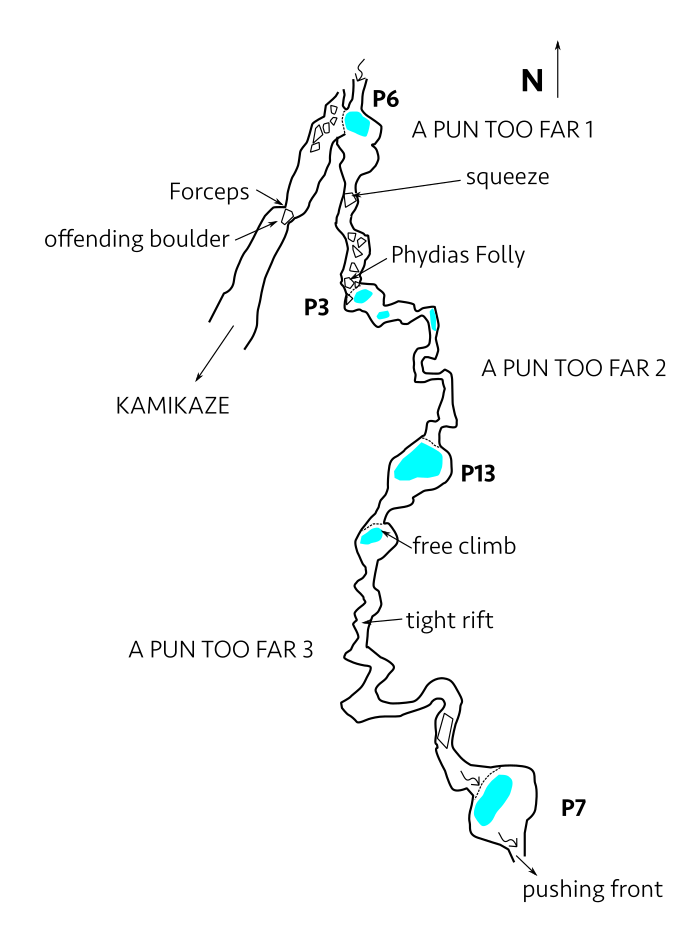
\includegraphics[width=\textwidth]{images/2014/tanguy-2014/puntoofar.png}}
\caption{The grade 1 survey of \protect\passage{A Pun too far} streamway was drawn in the Underground Camp logbook --- Tanguy Racine}
\label{Notebook pun too far}
\end{figure}

Being early birds again, we cooked breakfast under Rhys's unimpressed eye. `They have yet to understand the principle of camp faff' is what I believe was written down in the Underground Logbook. Oblivious to the disapproving gaze, we set off a third time. We had chisel and crowbar at the ready, and would crack this boulder open with a mailed fist...

We managed the crawl ever more swiftly, as every turn and angular pebble became more familiar, squeezed past the Forceps with ease, descended the cascade pitch, wriggled through the rift, and emerged on the false floor. Without wasting any moment, we started hammering at the rock. 

`If we could get rid of that nodule, then maybe,..., put the crowbar here.... heave.... hammer.... push, no pull. What about this nodule? Chisel... heave now, it's moving! HEAVE?'


To no avail. The boulder was well and truly jammed. It was marginally reduced in size, and rock powder was in the air.

I bit back a sigh. I was warm now and panting from the effort. The dribble of the water below was more tantalising by the instant. 

In a stroke of genius, Aileen started `If we could secure the boulder, I mean it \emph{is} jammed, there might be enough space to squeeze underneath, all we'd have to do is... more chiselling to enlarge the pitch head'.
I knew this pitch head would be awkward whatever the outcome: very tight, and with a spear of rock about a metre underneath. But I started chiselling madly at the rock. Now that the plan we had seemed to be functional, the thrill of exploration drove my hand down, and down, and down again with a renewed energy. In minutes, a few good sized nodules had been chipped away. In the end, it needed a few more furious blows before Aileen's helmet disappeared underneath.

I eagerly followed, managed the squeeze by hanging my ascending gear from the long cow's tails. I was elated when my feet touched the floor. There we were, back in the little stream and the chase for the lead was on.


\begin{marginfigure}
\frame{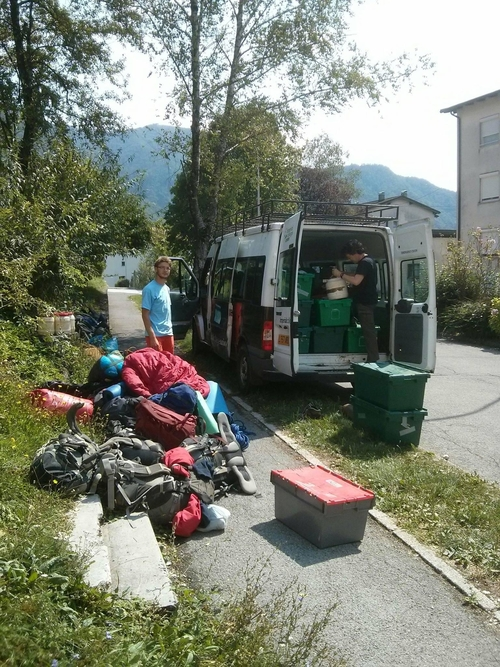
\includegraphics[width=\linewidth]{images/2014/tanguy-2014/minibus_packed}}
\label{packing the bus}
\caption{Repacking the minibus at the end of expedition is always easier, most of the food has been eaten!  --- Tetley}
\end{marginfigure}


The rift we then followed is very much controlled by an oblique fault. We followed the passage down for a few turns until it seemed to close down again. However, shimmying upwards again lead to an opening... is that the splashing of water droplets down a cascade? The awkward crawl led to yet another pitch head!

And this one was larger than the two small drops we'd found during the earlier days. Again, muttering a curse, we realised that we were lacking rope to descend it. This drop however represented the first big opening of the passage after the breakthrough, so we shook hands on the discovery, and surveyed all the way back to the jammed boulder.

Seeing as we hoped to bottom the pitch on the morrow and what we had found amounted to a few tens of metres, we carried on with the name \passage{A Pun Too Far}. We surveyed the rift, and at the pitch head, thought of a name for the very tight pitch head. We had chiseled away most of the rock and \passage{Phydias's folly} seemed appropriate.

For a third time, we went back to camp. We met Rhys and Sarah there. From what I heard, they'd pushed something horrible. Worse they'd taken the camera we had only to take photographs of a thick vegetable soup. That's another story altogether. They would be going up on the morrow. We wouldn't yet, we had a pitch to bottom...

And so we did, by noon on the fourth pushing trip, we were down the pitch. To our dismay it all closed down again, but we followed the rift, free climbing a 2 metre drop into a small pool, down more rift. It didn't end, there was always more. It twisted and twisted until again it opened up, into a circular seven metre drop. It was getting late on the last trip we intended to do, so we turned back then, leaving a storming lead for the following year. Before leaving the limit of the exploration, we has a small photo session.


\begin{marginsurvey}
	\includegraphics[width= \linewidth]{"images/little_insets/pun_too_far_inset".pdf}
	\caption[A Pun Too Far]{Plan view of the \protect\passage{Kamikaze} crawl leading to  \protect\passage{A Pun Too Far} streamway --- Slovenian National Grid EPSG 3794}
\end{marginsurvey}

The fourth morning was the worst, knowing there was no escaping the 550metre ascent. The long stay underground was wearing on me know, and the long pitches finished me. My footloop snapped in the \passage{Urinal Series}, this setback gave a little rest, and with Aileen's spare dyneema footloop, I raced upwards. All too soon, the final squeezes were behind. One last scramble up the scree slope. Daylight, warmth and a can of beer!
\mydelimiter
\newpage
\section{Epilogue}

`Hey ho!' Silence. 

`Does it go?', `do you want some tea?', `yes', `cow?', `no'...

`Yes the cave goes, it always goes, the mountain is hollow after all.'

`Shall we enter the survey data right away?',

`What a question... Of course'. Little by little the 150 metres or so of passage are added to the grand survey. What a joy to see four days worth of work take shape before one's eyes! Where does it head to? Is it blank mountain? 

As ever we raise more questions than we actually answer.

There lies the thrill of exploration: more people have been to the Moon than in the passage we found. To compound matters, this was the my ultimate caving trip before Derig-day when we would put the cave to sleep for another year by packing up camp \passage{X-Ray} and finally head down to \passage{Tolmin} and celebrate before the very long journey home. 

\name{Tanguy Racine}

%\begin{pagefigure}
%\checkoddpage \ifoddpage \forcerectofloat \else \forceversofloat \fi
%\centering
%\frame{\includegraphics[width=\textwidth]{"images/2014/tanguy-2014/area_n_sunrise".jpg}}
%\caption{From the summit of \protect\passage{Tolminski Kuk},the unobstructed view of the scenic \protect\passage{Julian Alps} reminds us why we choose to go back to Slovenia every Summer   --- Tanguy Racine}
%\label{fig:plateau}
%\end{pagefigure}



